% Chapter 1

\chapter{Final version} % Main chapter title

\label{Chapter5} % For referencing the chapter elsewhere, use \ref{Chapter1} 

Here will be explained the features of the final version, and how we are arrived at it.

\section{Functional requirements}

The last version (from now "gAn Web v3") is a modified version of the intermediate version. 
The second version's modification come from two sources: some adding requirements are proposed from the pilot users (that are also supervisors) and some else come from the tests made with the generic users; The first group of  adding requirements (the ones proposed by the supervisors) are the following:

\begin{enumerate}
%1 chose analysis new way
\item 
The main kinds of analysis are now more clear: they are around 15, and they are     quite stable (their goals, so their input and expected output are quite stable, but still we'll probably modify the algorithmic ways in which these goals are achieved; from the point of view of the web interface the situation us quite stable). Their roles and when they are useful is now steadily fixed (more precisely: we are pretty sure about the role of the existing analysis, but in the future we can add more analysis..). Each user, according on his task, knows (should know) in every moment which analysis fits better the situation, so, the best solution is allows the user to choose the type of the analysis through a dropdown menu directly in the main page (exactly like he chooses the run number). At this point the possibility of choose the gAn version is useless, because the definitive version of gAn include all the existing types of analysis. 

%2 single vs multiple
\item 
The kind of use of this software is quite different if you decide to work with a single run or a group of runs, so is better if at the beginning (at the application starting) the user chooses directly if he wants work with a single run or more than one. 

If the user works with a single run the focus is mainly on the "exploration" of the information in the data, with the multiple runs the focus is more on the possibility to compare and see what is different.

In the second case (more then one) is better to tell if the runs are a range (form N to M, all the runs between) or a group of non-consecutive runs (it can be useful, because of the feasibility to compare non-consecutive runs can be interesting). If the user is interested in a group of runs that are not a range, the previous solution of multiple runs separated by a comma is not a good idea: often in these cases the researched runs are little consecutive groups, so a list of ranges. It is better if the user can have an input area (like a sheet) in which he can put the intervals, divided in different lines (or other separators).

%3 don't choose root version
\item
There is an effort in the developing of the whole project to make it independent of the Root version, so the interface won't ask to the user to choose a Root version anymore. 

\end{enumerate}
 
Furthermore, the version version with this last requirements was tested with the users: the developer studied their behavior observing them at work with the existing version, listening to their comments, and asking them opinion and information. The impact of the debut with the users highlights some problems to be overcome, and also provide some interesting ideas: from the analysis and the solution of these problems and from the user's proposals the requirements of the last version was defined. The problems observed (and for each the proposed solution) are the following:

\begin{enumerate}
\item 
It is important to help the user in some way to choose the run number: the user needs a view on the logbook of the run, that is a text in which there are information about each run number divided by date.

\item
Actually nobody use the button to modify the dimension of the images: they all use the biggest version.. is better to remove (or move in a less central place) this dropdown menu. A similar reasoning can be done for the dropdown that allows the user to switch between the vertical and carousel menu (everybody use vertical, clearly at this point the carousel version isn't useful). Also nobody us the run selector to choose which image see: they prefer base themselves on the image's title.. at this point a surely better solution is to create a selector with the image's titles, precisely a group of check-boxes, each with the title of an image as label, using that the user can select one or more (or all if he wants) images.  

\item
The read of the textual output takes too much time: it can be improved highlighting the most important parts (or better, the most important parts for the selected type of analysis)

\item
The user needs to choose by the configuration page the degree of precision (the minimal error) of the x-axis (the time related axis) of each time-related values images. This parameter seemed to be not very important and in the second version actually there wasn't, but almost all the users modify it quite often (manually), and verbally ask for the possibility to set it through the interface. So is better to let them to do it by the interface

\end{enumerate}

\section{Non-functional requirements}

There is another special requirement emerged in this version, not strictly related to the common behavior of the interface but quite important: the machine  used as server is also used for the testing of single analysis when they are written; sometimes these analysis crashes (quite normal in a test phase), and they remain in a "hung up" state, without doing nothing but occupying Ram memory, and if the blocked application are numerous that can be a problem for the performances of the machine. To ensure a correct behavior gAn Web must check this situation at starting and eventually resolve it.

\section{Scenario based functional analysis}
Following we can show some examples able to explain how the typical interaction must work in the definitive version:

\begin{enumerate}

\item
Let's suppose a very common situation in a shift: 
In the shift is running the run NNNN. The shifter wants to calculate the temperature of some particles with a (complex) process based on the shape that they create on a sensor (the basic idea is: if a particle is hotter, its speed is bigger, it can escape more easily from a magnetic trap, and the sensor can observe more particles outside the trap. At this point the software tries to fit, with an exponential function, the shape of the signal that the sensor shows as output, and through the integral of the slope of this exponential function can estimate the temperature of the particle).
 
The user chooses the single analysis, insert the run NNNN, select the kind of analysis called "TemperatureMeasurement", presses start;
The system shows to the user a textual output and some images: 
The textual output proposes a lot of information, but in the ninety five per cent of the cases the user is interested in only three parameters, that are clearly highlighted by a special font, a color and a visible border. 

The user must also check the image: there is the histogram of a signal, an a red line where the function is fitted. The user checks if the red line
has an exponential shape (if it is a straight line the situation is too aleatory and the data are not affordable); the user also check if the fit line is too long (it must be very little to accept the results of the analysis, because of physical reasons). 

Let's suppose that the fit function is a straight line: the user can retry the same analysis with a different setting: he return to the homepage (through the button "new analysis" on the navbar), he clicks "advanced setting" to modify the configuration, he insert a new value %TODO %TODO %TODO %TODO  THROUGH A input field of through a BOOTSTRAP SLIDER %TODO %TODO %TODO %TODO 
to have a more precise graph, in the hope to fit it better. At this point he can retry the previous algorithm (a more precise function will lead a slower computation but probably will give an affordable output)  

\item 
The user is interested in a two distinguished groups of runs, from 57001 to 57005 and form 57016-57020.
This situation is very common because most of the groups of measurements are repeated in two different slices of times (to be sure about the results).
In this case the user, after having selected "multiple runs", can click on "insert runs by Input Area" %TODO %TODO %TODO  CAMBIA IL NOME DEL BOTTONE!   
and an input area appears. In the area there are the value inserted the last time that the user used this function (we observe that is quite common repeat analyses with the same groups). The input is quite free: user can insert a group inserting the first and the last separated by a dash, a space, or a comma, and other group by changing the line (so each not empty line is a group). 
The user at this point confirm the input, and return on the homepage in which he can select the analysis and run the program. 

\item
The user is interested in a range of runs, from 58001 to 58010, to perform the same analysis and check if and how some values are varying. He can select multiple runs, insert the first and the last, select the analysis (the multiple runs analysis are taken from a different set from the single runs analysis).

\item
The user insert a run, and select an analysis names PMTs. This kind of analysis take information from a group of 14 sensors and produces in output (usually) seven images. The user often is not interested in all the seven images but in one or two. At this point, using the check-boxes selector he can select/deselect images to show (by default they are all selected).  

\end{enumerate}

\section{Prototypation}

Here is explained with some screen-shots how the final version looks like, and how does it work.

Login page:


\begin{figure}[H]
\centering
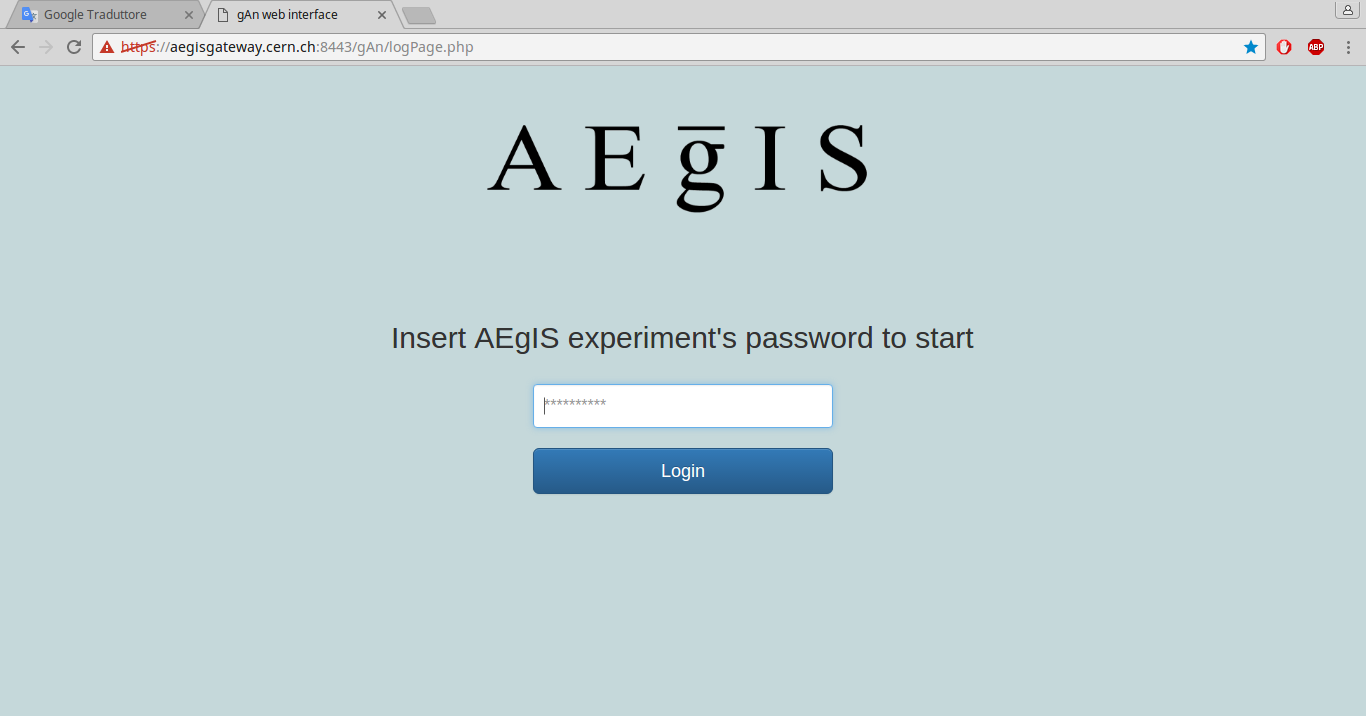
\includegraphics[scale=0.25]{LastLogin.png} 
\caption{The Login Page of gAn Web}
\end{figure}

First of all the login page: it is very simple, only one user exists (all the people in the AEgIS experiment are equal when they use this software, and no others experiments use this application) so only the password needs to be inserted, in order to ensure that only people who work in the experiment can use the software. We can see the typical objects taken from the Bootstrap's default graphic objects.


Home page, initial choice:

\begin{figure}[H]
\centering
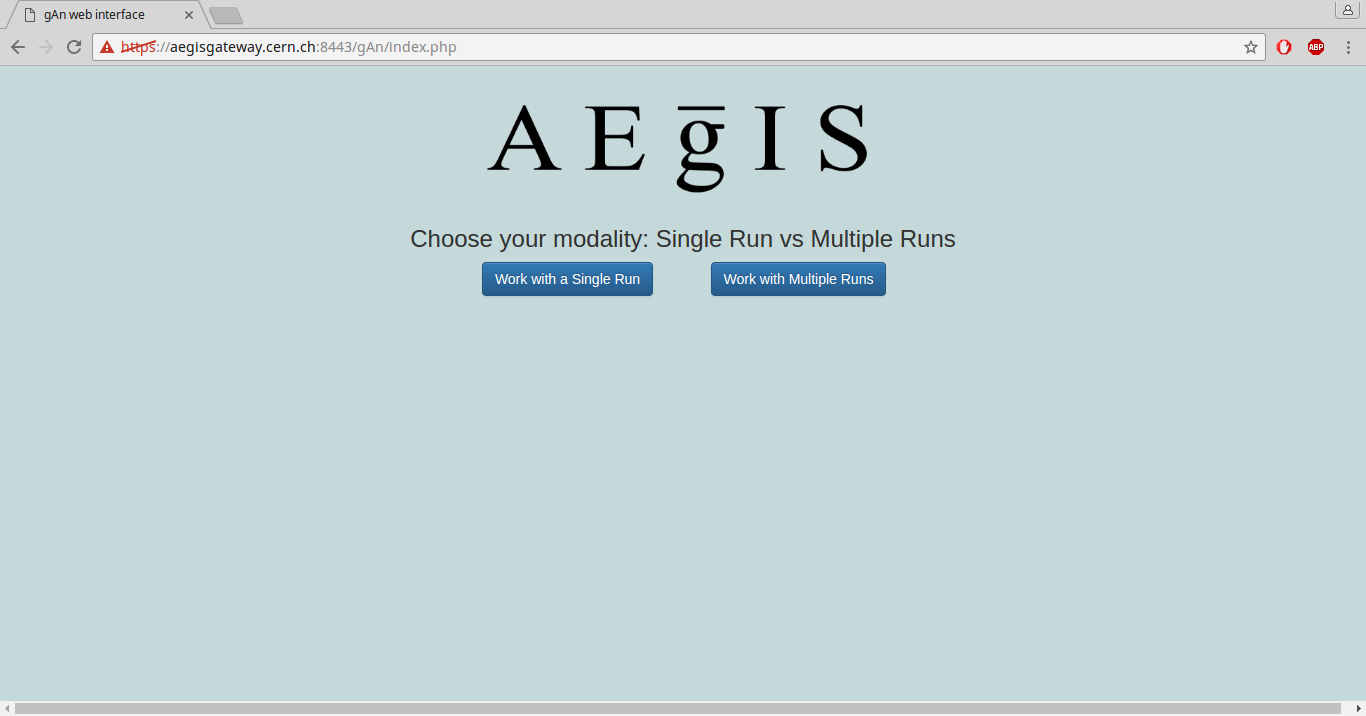
\includegraphics[scale=0.25]{LastInitialChoice.png} 
\caption{The first thing that a logged user sees}
\end{figure}
  
The neo-logged user can here choose if he is interested in a single run analysis of in a multiple runs one. These two situations are quite different, so the application work with them in two different ways.


Home page, differences between single and multiple runs:

Here we can see how the two modalities of work (single and multiple) appears: 
\begin{figure}[H]
\centering
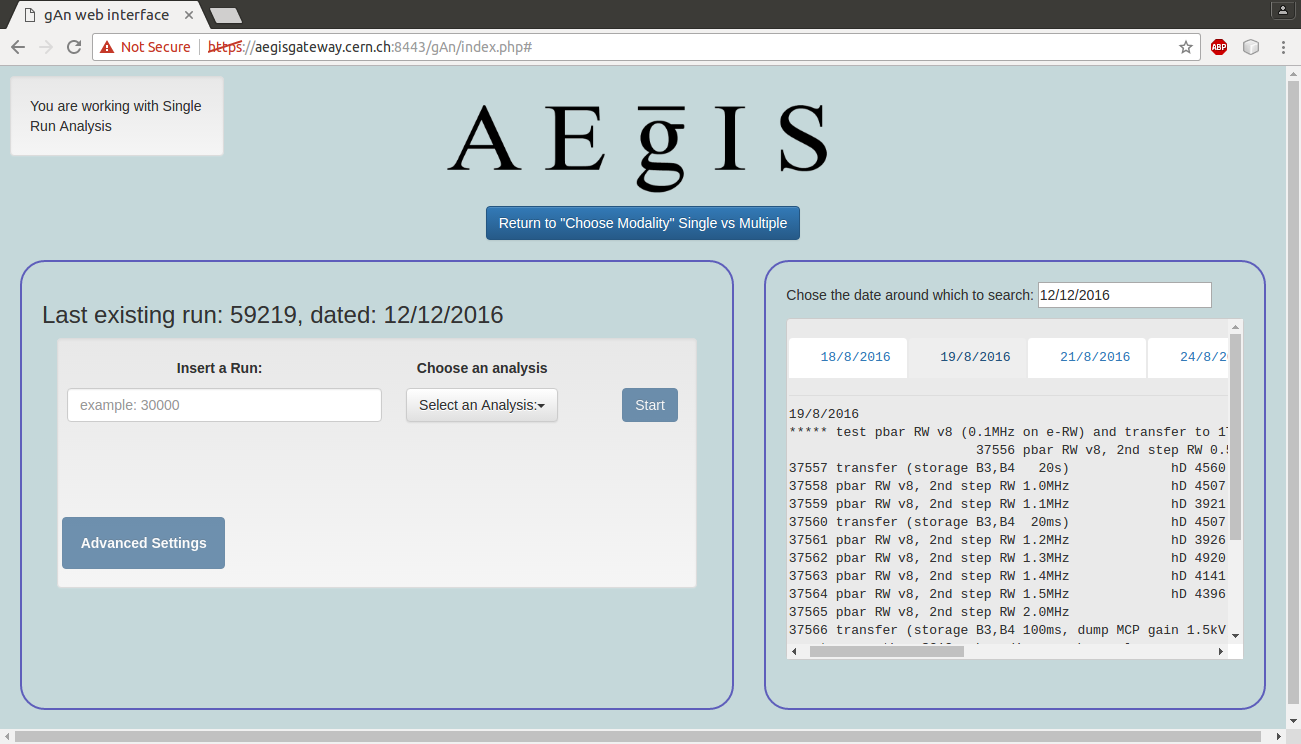
\includegraphics[scale=0.25]{LastSingle.png} 
\caption{The Homepage if the user chose Single run analysis}
\end{figure}

the single one is more simple, on the left of the screen the user inserts a run number and a kind of analysis. We can see the button related to access the configurator and modify the settings. On the right part of the screen there is a view on the runlog of the experiment. The user uses the right part when he wants more information about what run use to work (actually this situation is quire seldom). In the case the user can insert a date using a datepicker, the system opens some pages related to the days around that date and in each page shows the content of the logs related to this date. The log are always divided in runs, and for each run there are some informations and comments. At the moment this functionality is a mock-up (in is the only one mock-up of this document). On the  top-left of the screen there is always a little note with some information about the status of the program: this is a little cognitive aid. On the screen there is always wrote the last known run, because in most cases the users use it or the immediately previous one. 


\begin{figure}[H]
\centering
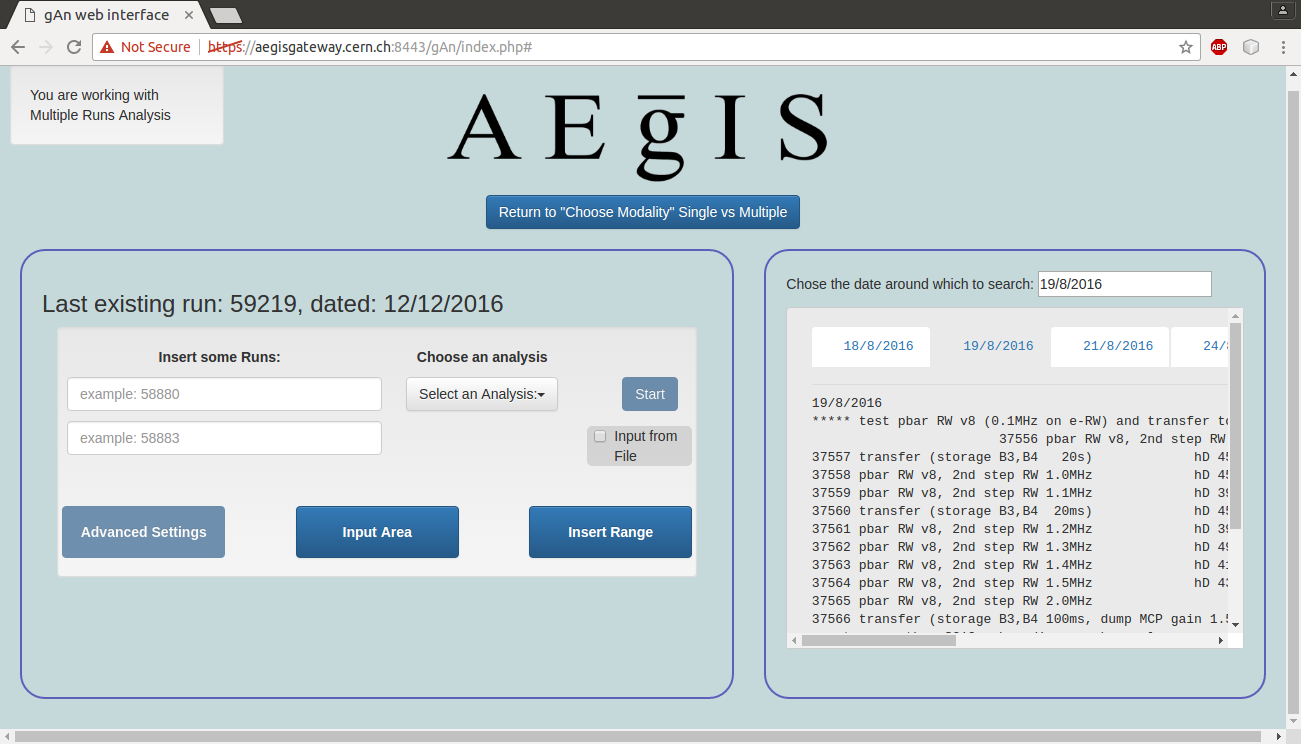
\includegraphics[scale=0.25]{LastMultiple.png} 
\caption{The Homepage if the user chose Multiple runs analysis}
\end{figure}    

The multiple runs modality is similar but more complex: in a standard situation the user inserts two runs, the first and the last. The alternative (less used) situation is the one in which the user, through the "Input Area" button insert a  list of groups of runs (this runs are written in a file, that the system is able to accept as input). This modality is sometimes useful, and can be activated with the check-box "Input from file". The activation of this modalities denies the access to the two input fields (you must only one way to insert runs..).
Following a little example of how the user can insert data through an Input Area:

\begin{figure}[H]
\centering
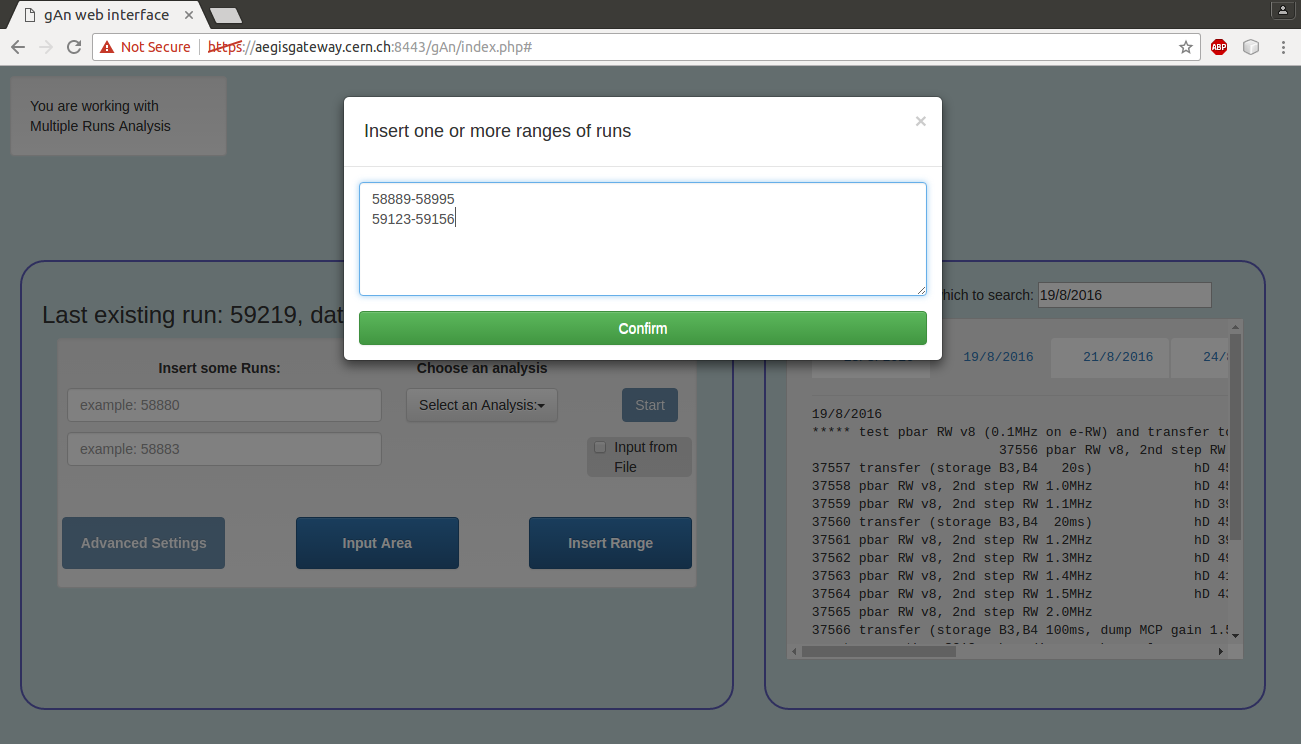
\includegraphics[scale=0.25]{LastMultipleRange.png} 
\caption{The Homepage if the user chose Multiple runs analysis}
\end{figure}   


Output: 

There are some innovation. The first one is the navbar: now the user can find here all the most important commands. Before there was more buttons, distributed in the screen, and during the tests the users had problems to found them and to understand their functionalities. Now the navbar is more clear and organized:

\begin{figure}[H]
\centering
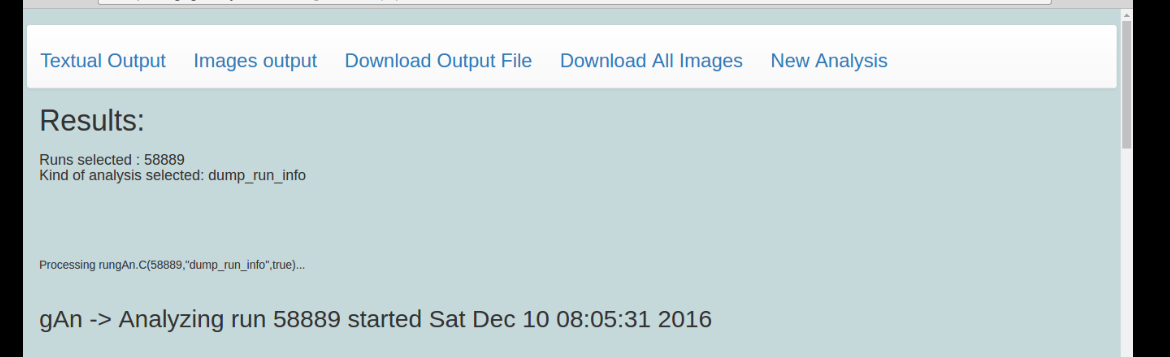
\includegraphics[scale=0.25]{LastNavbar.png} 
\caption{The output in textual version}
\end{figure}  


Textual Output:

\begin{figure}[H]
\centering
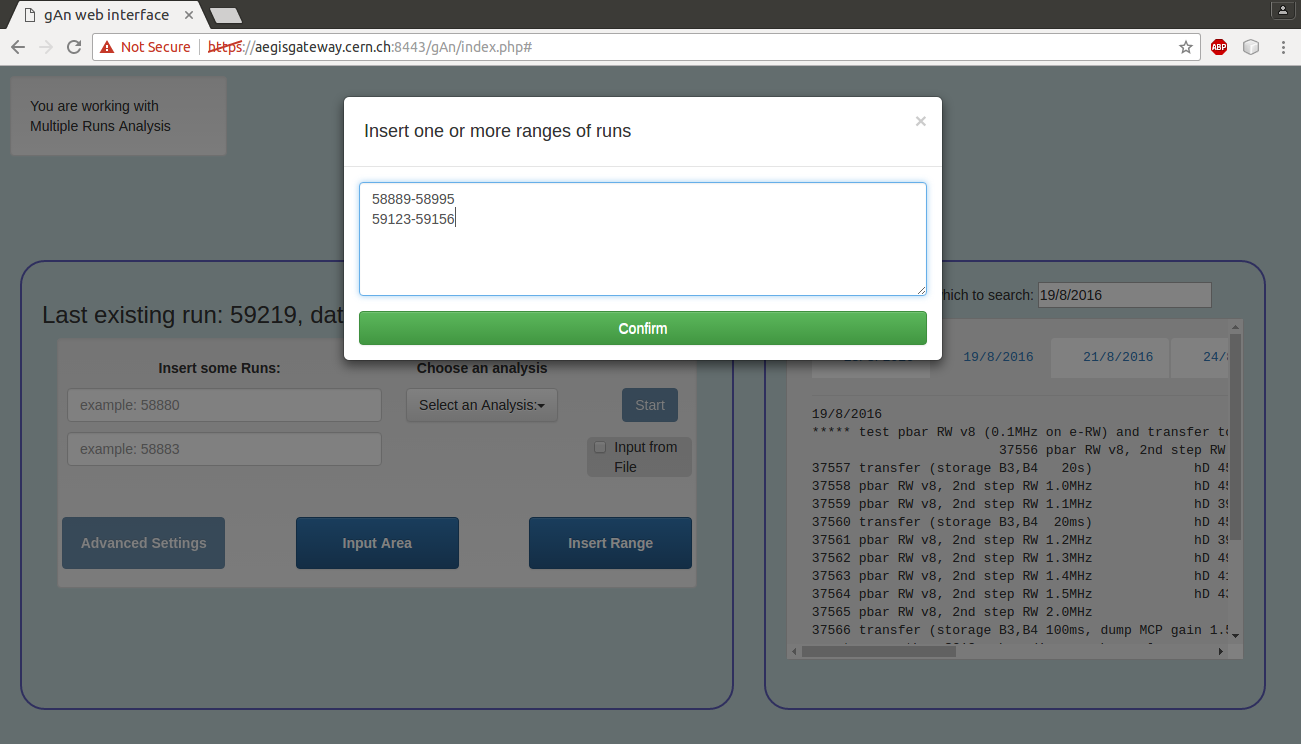
\includegraphics[scale=0.25]{LastMultipleRange.png} 
\caption{The output in textual version}
\end{figure}  

Here we can see out a textual output appears: there are more information, but in the 95 per cent of cases only a few are really useful, so they are highlighted with a special font and a big border (the hope is to use perceptive suggestions to advise the user about where to find what he searches). In this example we can see also some warnings: where something works wrong (or simply not perfectly) the system informs the user about the problem, with a red color, to ensure that he sees it. 

Images output:

\begin{figure}[H]
\centering
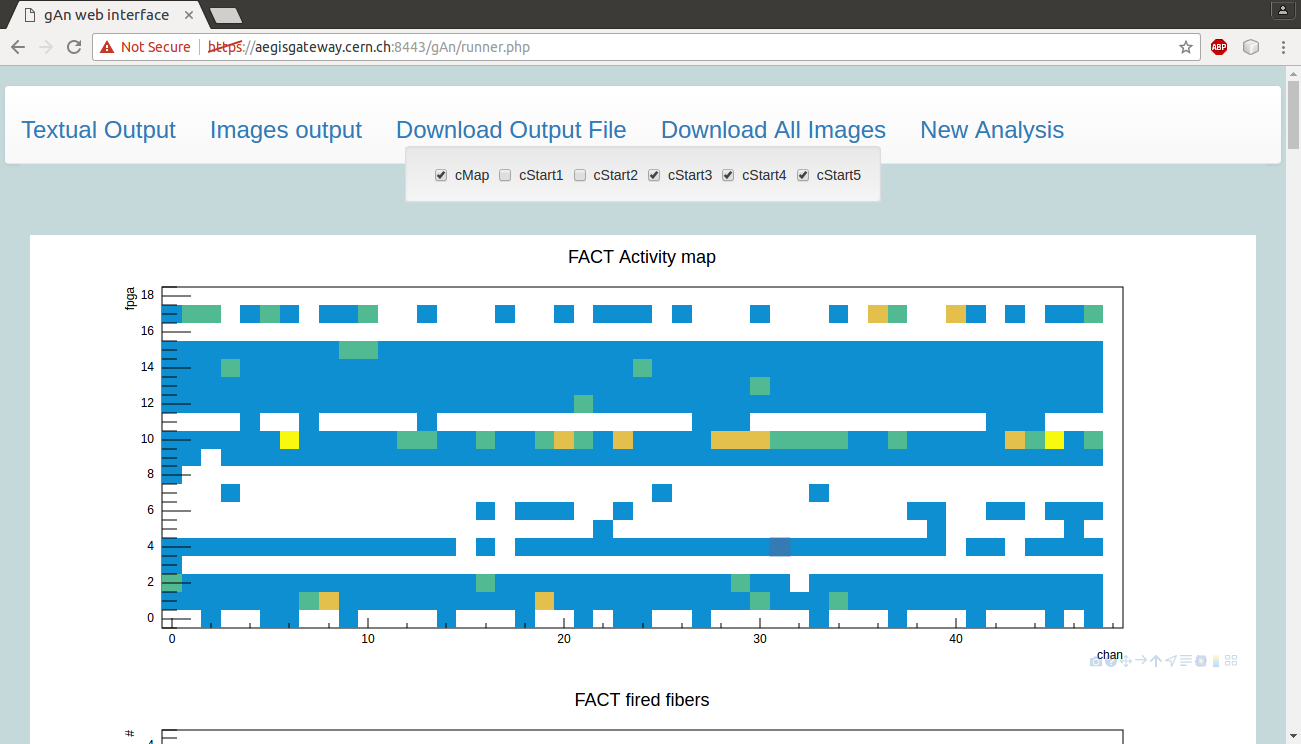
\includegraphics[scale=0.25]{ImageOutput.png} 
\caption{The output images}
\end{figure}  

Here we can see that there is no more the opportunity to select the dimension of the images (but still there is a zoom function in the image), or the layout, because none of the users never used these functionalities in the tests .. nor the possibility to choose a particular run of a group of images: this is because like discussed previous in this chapter the existing of the "kinds" of analysis makes this choice useless. Instead there is a list of check-boxes that is selected or deselected let the images appear and disappears. This feature is not important with 2 or 3 images, but sometimes the images are 7-8-9 so it is necessary.

Also in this case we observed that the users in most cases search in the images (almost) always the same information, so in some images the most important data (often they are dimension of peaks or integrals of spaces, or distances between peaks, or, in the case of charts with a time on the x-axis, auto-generated timelines about asynchronous events and triggers happened etc..) are directly written on the picture, like the following example:

\begin{figure}[H]
\centering
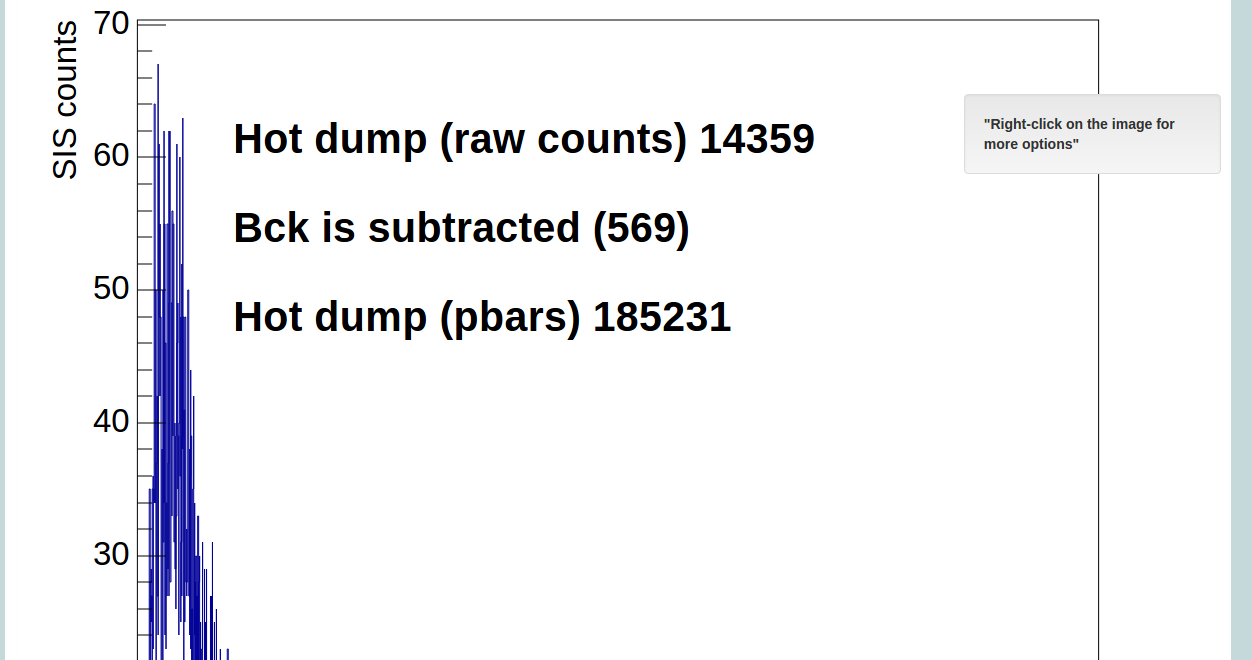
\includegraphics[scale=0.25]{LastImagenotes.png} 
\caption{Images with infos}
\end{figure}   

Still there is the opportunity to access more information right clicking on the graph, of modifying it in various ways for example showing the graph in three dimensions: 

\begin{figure}[H]
\centering
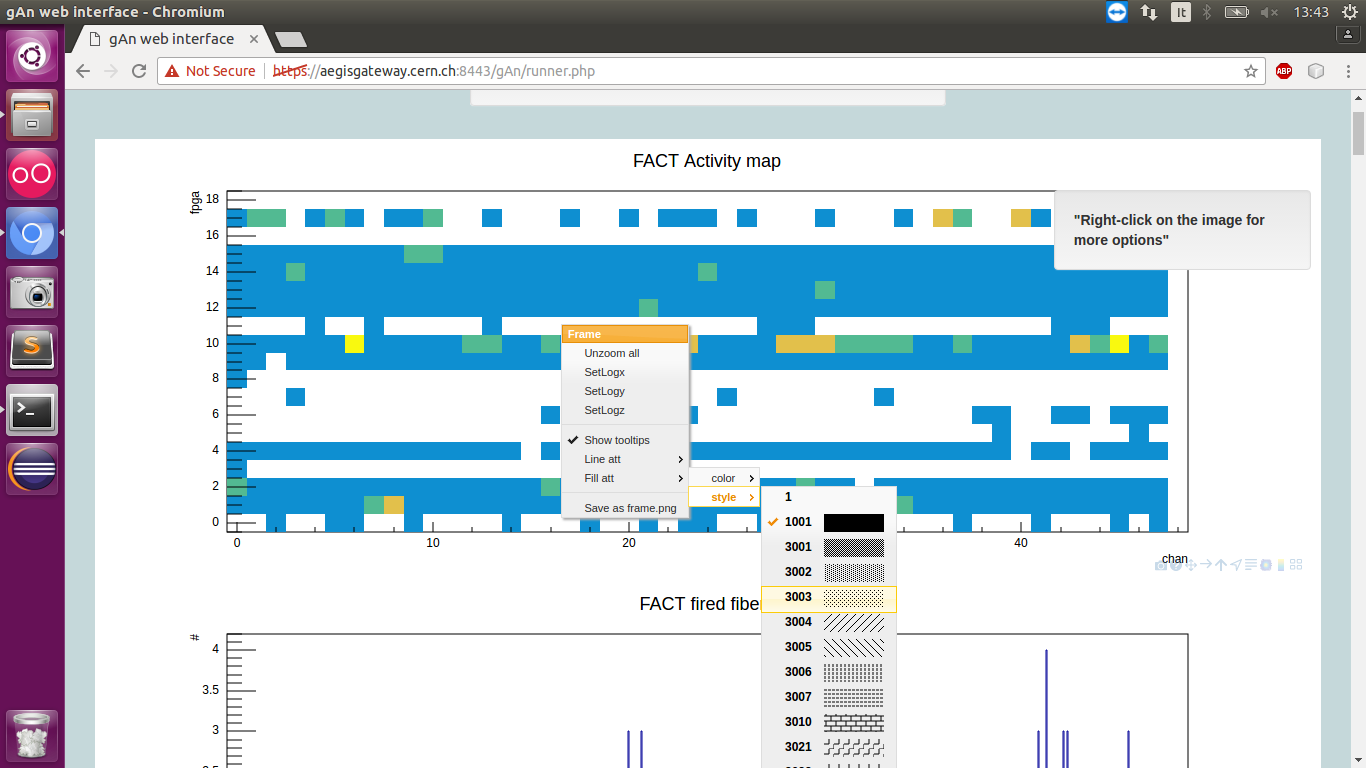
\includegraphics[scale=0.25]{LastImageOptions.png} 
\caption{Some options}
\end{figure}  

\begin{figure}[H]
\centering
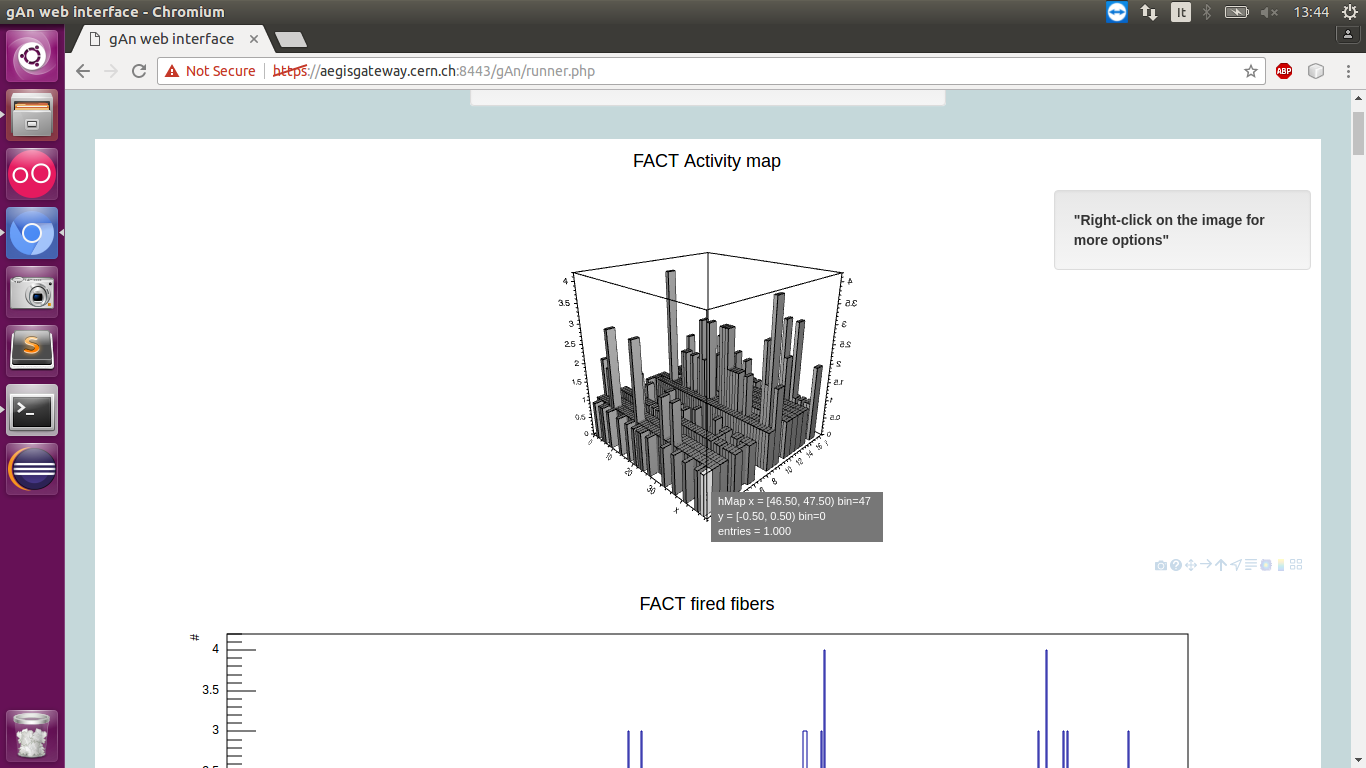
\includegraphics[scale=0.25]{LastGraphImage2.png} 
\caption{Other option}
\end{figure}  

Often the users in the tests had problems understanding that with a right click they could access these functionalities, so no there is a specific label on the right of the screen to inform them (this label is in fixed position, but became visible only if the user arrive with the scrollbar on the images):

\begin{figure}[H]
\centering
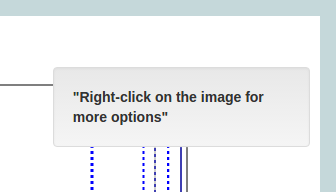
\includegraphics[scale=0.25]{LastImageLabel.png} 
\caption{Label to inform the user about a feature}
\end{figure} 

